\documentclass[tikz,border=2pt]{standalone}
\usepackage{amsmath,amssymb}
\usepackage{tikz}
\usetikzlibrary{arrows.meta,matrix}

\begin{document}
% Sarrus' rule for a 3x3 determinant: copy the first two columns to the right, add the three
% down-right diagonal products and subtract the three up-right ones.
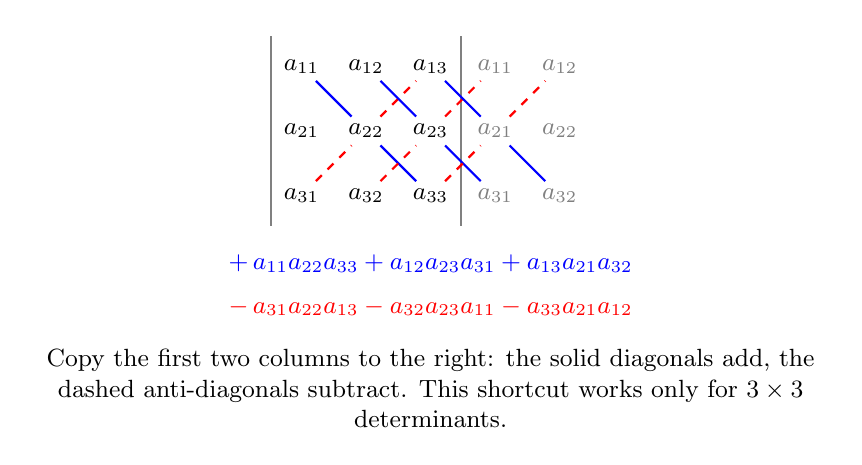
\begin{tikzpicture}[every node/.style={font=\small}]
	\matrix (S) [matrix of math nodes, nodes={minimum size=7.5mm, anchor=center}, column sep=2pt, row sep=2pt] at (0,0) {
		a_{11} & a_{12} & a_{13} & |[text=gray]| a_{11} & |[text=gray]| a_{12} \\
		a_{21} & a_{22} & a_{23} & |[text=gray]| a_{21} & |[text=gray]| a_{22} \\
		a_{31} & a_{32} & a_{33} & |[text=gray]| a_{31} & |[text=gray]| a_{32} \\
	};
	\draw[gray, thick] (S-1-1.north west) -- (S-3-1.south west);
	\draw[gray, thick] (S-1-3.north east) -- (S-3-3.south east);
	\foreach \s in {1,2,3} {
		\pgfmathtruncatemacro{\b}{\s+1}
		\pgfmathtruncatemacro{\c}{\s+2}
		\draw[blue, thick, shorten <=2.6mm, shorten >=2.6mm] (S-1-\s.center) -- (S-2-\b.center);
		\draw[blue, thick, shorten <=2.6mm, shorten >=2.6mm] (S-2-\b.center) -- (S-3-\c.center);
		\draw[red, thick, dashed, shorten <=2.6mm, shorten >=2.6mm] (S-3-\s.center) -- (S-2-\b.center);
		\draw[red, thick, dashed, shorten <=2.6mm, shorten >=2.6mm] (S-2-\b.center) -- (S-1-\c.center);
	}
	\node[blue, anchor=north, align=center] at (0,-1.45) {$+\,a_{11}a_{22}a_{33}+a_{12}a_{23}a_{31}+a_{13}a_{21}a_{32}$};
	\node[red, anchor=north, align=center] at (0,-2.0) {$-\,a_{31}a_{22}a_{13}-a_{32}a_{23}a_{11}-a_{33}a_{21}a_{12}$};
	\node[anchor=north, align=flush center, text width=10cm] at (0,-2.65) {Copy the first two columns to the right: the solid diagonals add, the dashed anti-diagonals subtract. This shortcut works only for $3\times3$ determinants.};
\end{tikzpicture}
\end{document}
